\newpage


\section{Slope and Flux Limiters}




%===========================================
\subsection{Slope Limiters}
%===========================================

Slope limiters are employed because issues arise around numerical schemes because of their discrete nature.
For example, a non-limited piecewise linear advection scheme will produce oscillations around jump discontinuities.
See \textbf{Godunov's Theorem}:



\begin{displayquote}
	Linear numerical schemes for solving partial differential equations (PDE's), having the property of not generating new extrema (monotone scheme), can be at most first-order accurate.
\end{displayquote}

So the idea is to compute the slope in way that is useful for us based on the current situation of the gas state that we're solving for.

The choice of the slope can be expressed via a function $\phi(r)$.
For simple advection, we are solving the equation:

\begin{align}
	\U_i ^{n+1} &= 
		\U_i^{n} +  \frac{\Delta t}{\Delta x} \left( \F_{i-\half}^{n+\half} - \F_{i+\half}^{n+\half} \right) \label{eq:advection}
\end{align}


If we assume that the states $\U_i$ are piecewise linear, i.e.
\begin{align}
	\U(\x) = \U_i(\x_i) + \mathbf{s}\cdot (\x - \x_i) \quad \text{ for } \x_{i-\half} \leq \x \leq \x_{i+\half} \label{eq:advection-slope}
\end{align}


then the expression for the fluxes is given by


\begin{align*}
	\F_{i-\half}^{n+\half} &= 
		\begin{cases}
			\V_{i-\half} \cdot \U_{i-1}^n +  \frac{1}{2} \V_{i-\half} \cdot\mathbf{s}_{i-1}^n (\Delta \x -  \V_{i-\half} \Delta t)
			 	& \quad \text{for } \V \geq 0 \\
			\V_{i-\half} \cdot \U_{i}^n -\frac{1}{2} \V_{i-\half} \cdot \mathbf{s}_{i}^n (\Delta \x + \V_{i-\half} \Delta t)
				& \quad \text{for } \V \leq 0 \\
		\end{cases} \\
	\F_{i+\half}^{n+\half} &= 
		\begin{cases}
			\V_{i+\half} \cdot \U_{i}^n +  \frac{1}{2} \V_{i+\half} \cdot\mathbf{s}_{i}^n (\Delta \x -  \V_{i+\half} \Delta t)
			 	& \quad \text{for } \V \geq 0 \\
			\V_{i+\half} \cdot \U_{i+1}^n -\frac{1}{2} \V_{i+\half} \cdot \mathbf{s}_{i+1}^n (\Delta \x + \V_{i+\half} \Delta t)
				& \quad \text{for } \V \leq 0 \\
		\end{cases} \\		
\end{align*}




We can now insert a more general expression for the slopes: Let 
\begin{align}
	\theta_{i-\half} = \begin{cases} +1 \quad \text{ for } \V \geq 0 \\ -1 \quad  \text{ for } \V \leq{0} \end{cases}
\end{align}

Then



\begin{align}
	\Delta x_{i-\{0, 1\}} \mathbf{s}_{i-\{0,1\}} 
		&= \frac{1}{2} \Delta x \left[ (1 + \theta_{i-\half}) \mathbf{s}_{i-1}^n + (1 - \theta_{i-\half})  \mathbf{s}_{i}^n \right]  \\
	&\equiv \phi(r_{i-\half}^n) (\U_i^n - \U_{i-1}^n ) \\
	r^n_{i-\half} &= \begin{cases}
		\frac{\U_{i-1}^n - \U_{i-2}^n}{\U_{i}^n - \U_{i-1}^n} 	\quad \text{ for } \V  \geq 0 \\
		\frac{\U_{i+1}^n - \U_{i}^n}{\U_{i}^n - \U_{i-1}^n} 	\quad \text{ for } \V  \leq 0 \\
	\end{cases} 
\end{align}

This defines $\phi$, which will be discussed later. Finally:

\begin{align}
	\F_{i-\half}^{n+\half} = 
		&\frac{1}{2} \V_{i-\half} \left[  (1 + \theta_{i-\half}) \U_{i-1}^n + (1 - \theta_{i-\half})  \U_{i}^n \right] +\nonumber\\
		&\frac{1}{2}| \V_{i-\half} | \left( 1 - \left| \frac{\V_{i-\half} \Delta t}{\Delta x} \right| \right) \phi(r_{i-\half}^n) (\U_i^n - \U_{i-1}^n ) \label{eq:advection_phi1-limiters}\\
	\F_{i+\half}^{n+\half} = 
		&\frac{1}{2} \V_{i+\half} \left[  (1 + \theta_{i+\half}) \U_{i}^n + (1 - \theta_{i+\half})  \U_{i+1}^n \right] +\nonumber\\
		&\frac{1}{2}| \V_{i+\half} | \left( 1 - \left| \frac{\V_{i+\half} \Delta t}{\Delta x} \right| \right) \phi(r_{i+\half}^n) (\U_{i+1}^n - \U_{i}^n ) \label{eq:advection_phi2-limiters}
\end{align}







Depending on our choice of $\phi$, we can get different slopes. Here for positive velocity only, and for $r = r_{i-\half}$:

\begin{align*}
	\phi(r) & = 0 \rightarrow \mathbf{s}_i = 0 
		&\text{ No slopes; Piecewise constant method.}\\
	\phi(r) & = 1 \rightarrow \mathbf{s}_i = \frac{\U_{i} - \U_{i-1}}{\Delta x} 
		&\text{ Downwind slope (Lax-Wendroff)} \\
	\phi(r) & = r \rightarrow \mathbf{s}_i = \frac{\U_{i-1} - \U_{i-2}}{\Delta x} 
		&\text{Upwind slope (Beam-Warming)} \\
	\phi(r) & = \frac{1}{2} (1 + r) \rightarrow \mathbf{s}_i = \frac{\U_{i} - \U_{i-2}}{2 \Delta x} 
		&\text{ Centered slope (Fromm)} \\
\end{align*}



Note that taking the downwind slope is very different from doing downwind differencing!
We only use the downwind value to estimate the state inside the cell, not to compute derivatives.



As was said before, these kinds of slopes will introduce oscillations around jump discontinuities in the advected quantity.
See Godunov's theorem and figure \ref{fig:advection-pwlin-four-shapes-fixed-positive-vel}.



\begin{figure}
	\centering
	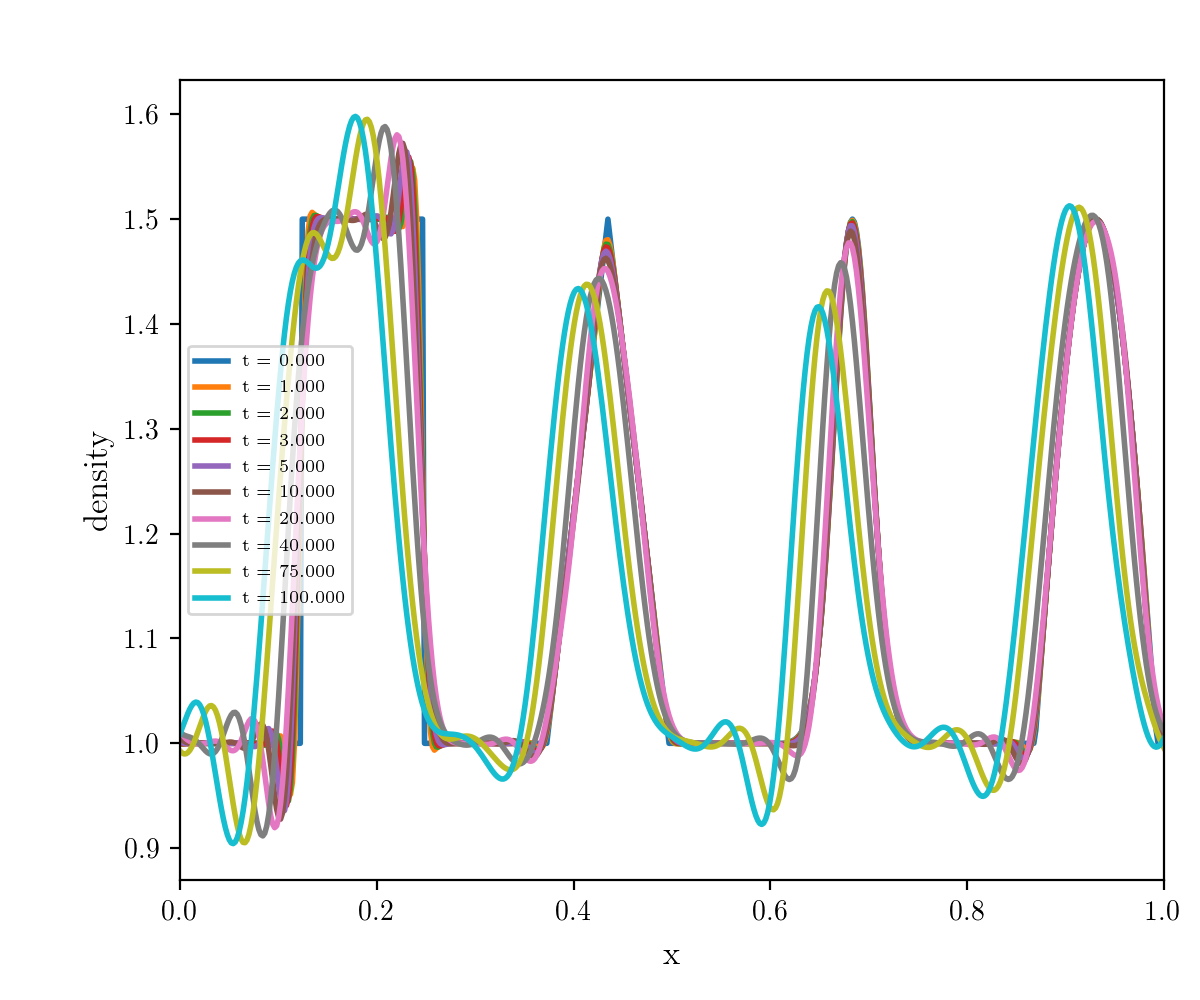
\includegraphics[width=.9\textwidth]{./figures/advection-pwlin-four-shapes.png}%
	\caption{
		\label{fig:advection-pwlin-four-shapes-fixed-positive-vel}
		Piecewise linear advection with positive fixed global velocity $v_x = 1$ at different times. 
		$C_{CFL} = 0.9$,  $nx = 100$.
		The oscillations are a natural consequence according to Godunov's theorem.
	}
\end{figure}

















%===========================================================
\subsubsection{What slope limiters have in common}
%===========================================================



So the idea behind slope limiters is to find an expression to \textbf{monotonize} the states, i.e. to be \textbf{Total Variation Diminishing (TVD)}.
A method is TVD if:

\begin{align}
	TV(\U^n) &\equiv \sum_j | \U_{j+1} - \U_j | \\
	TV(\U^{n+1}) &\leq TV(\U^n) \quad \Leftrightarrow \quad \text{ method is TVD }
\end{align}





Remember, we express the slopes with the function $\phi(r)$, where 

\begin{align*}
	r^n_{i-\half} &= \begin{cases}
		\frac{\U_{i-1}^n - \U_{i-2}^n}{\U_{i}^n - \U_{i-1}^n} 	\quad \text{ for } \V  \geq 0 \\
		\frac{\U_{i+1}^n - \U_{i}^n}{\U_{i}^n - \U_{i-1}^n} 	\quad \text{ for } \V  \leq 0 \\
	\end{cases}
\end{align*}.

$r$ is the ratio of the slopes, a measure of the ``curvature'', or ``monotonicity'' in that place.
To remove oscillations, we want to go back to a first order expression (piecewise constant expression) when we find an oscillation, i.e. when the numerator and denominator have different signs.
We get the piecewise constant expression for $\phi(r) = 0$

$\Rightarrow$ For slope limiters, we must have $r < 0 \Rightarrow \phi = 0$


Other restrictions follow from the constraint that the method should be TVD and continuous (see \cite{swebyHighResolutionSchemes1984}):

\begin{align}
	r \le& \phi(r) \le 2r 	&&	 0  \le r \le 1 \label{eq:TVD-consequence-first}\\
	1 \le& \phi(r) \le r 	&&	 1 \le r \le 2 \\
	1 \le& \phi(r) \le 2 	&&	 r > 2  \label{eq:TVD-consequence-last}\\
	& \phi(1) = 1 &&\\
\end{align}



Effectively, this defines regions in the $r-\phi(r)$ diagram through which the limiters are allowed to pass such that they are still TVD (fig \ref{fig:limiters-r-phi}) 





Popular limiters are:
\begin{flalign}
	\text{Minmod} 								&&\quad \phi(r) &= \mathrm{minmod}(1, r)\\
	\text{Superbee} 							&&\quad \phi(r) &= \max(0, \min(1, 2r), \min(2, r)) \\
	\text{MC (monotonized cenral-difference)} 	&&\quad \phi(r) &= \max(0, \min ((1+r)/2, 2, 2r))\\
	\text{van Leer}								&&\quad \phi(r) &= \frac{r + |r|}{1 + |r|}
\end{flalign}

where

\begin{align}
	\mathrm{minmod}(a, b) = 
		\begin{cases}
			a	& \quad \text{ if } |a| < |b| \text{ and } ab > 0\\
			b	& \quad \text{ if } |a| > |b| \text{ and } ab > 0\\
			0	& \quad \text{ if } ab \leq 0\\
		\end{cases}		
\end{align}



Their behaviour is shown in fig. \ref{fig:limiters-r-phi}.



\begin{figure}[H]
	\centering
	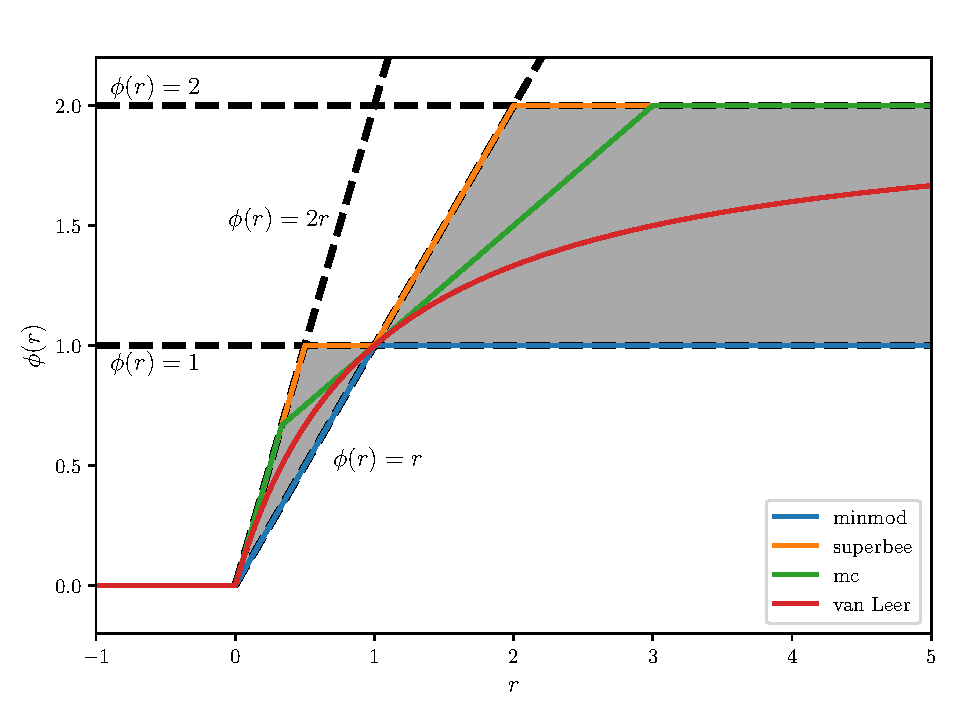
\includegraphics[width=.9\textwidth]{./figures/limiters.pdf}%
	\caption{
		\label{fig:limiters-r-phi}
		The behaviour for different slope limiters. The grey zone is the zone allowed by the conditions \ref{eq:TVD-consequence-first}  - \ref{eq:TVD-consequence-last}.
	}
\end{figure}








%===========================================================
\subsection{ Implemented Slope Limiters}
%===========================================================


The choice of the slope can be expressed via a function $\phi(r)$ (see eqns. \ref{eq:advection_phi1-limiters}, \ref{eq:advection_phi2-limiters}) with 

\begin{align*}
	r^n_{i-\half} &= \begin{cases}
		\frac{\U_{i-1}^n - \U_{i-2}^n}{\U_{i}^n - \U_{i-1}^n} 	\quad \text{ for } v  \geq 0 \\
		\frac{\U_{i+1}^n - \U_{i}^n}{\U_{i}^n - \U_{i-1}^n} 	\quad \text{ for } v  \leq 0 \\
	\end{cases}
\end{align*}.


Possible limiters are:
\begin{flalign}
	\text{Minmod} 								&&\quad \phi(r) &= \mathrm{minmod}(1, r)\\
	\text{Superbee} 							&&\quad \phi(r) &= \max(0, \min(1, 2r), \min(2, r)) \\
	\text{MC (monotonized cenral-difference)} 	&&\quad \phi(r) &= \max(0, \min ((1+r)/2, 2, 2r))\\
	\text{van Leer}								&&\quad \phi(r) &= \frac{r + |r|}{1 + |r|}
\end{flalign}

where

\begin{align}
	\mathrm{minmod}(a, b) = 
		\begin{cases}
			a	& \quad \text{ if } |a| < |b| \text{ and } ab > 0\\
			b	& \quad \text{ if } |a| > |b| \text{ and } ab > 0\\
			0	& \quad \text{ if } ab \leq 0\\
		\end{cases}		
\end{align}